\section{Pruebas y análisis de robustez en diferentes redes}

Las redes que se van a estudiar son:

\begin{enumerate}
    \item Red A: Red libre de escala 8000 nodos
    \item Red B: Red de mundo pequeño 5000 nodos, probabilidad de reconexión 10\%
    \item Red C: Red aleatoria 1991 nodos
    \item Red D: Red obtenida de bacteria C.elegans
    \item Red E: Red fractal (1,3)-flower
\end{enumerate}

\subsection{Pruebas en red libre de escala}

\begin{figure}[H]
    \centering
    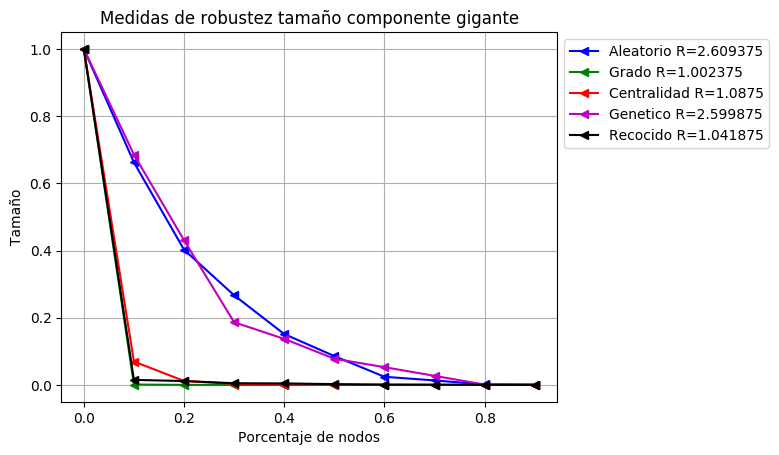
\includegraphics[scale=0.7]{Capitulo5Robustez/imagenes/grafica_GC20180512_143117ScaleFree8000Nodes.png}
    \caption{Medida componente de gigante}
\end{figure}


\begin{figure}[H]
    \centering
    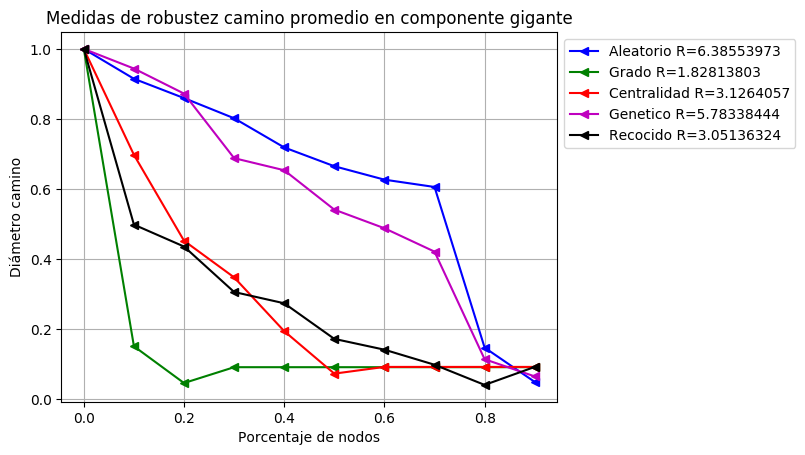
\includegraphics[scale=0.7]{Capitulo5Robustez/imagenes/grafica_APL20180512_143117ScaleFree8000Nodes.png}
    \caption{Medida componente de promedio de camino más cortos}
\end{figure}

En las redes libres de escala, las medidas indican que la red pierde sus propiedades estructurales más rápidamente con los ataques de grado y centralidad. Esto se debe a que en gran medida los hubs, son los que se encuentran entro de los caminos más cortos entre cualquier par de nodos.

Los ataques genético y recocido presentan una efectividad intermedia de daño.


\subsection{Pruebas red de mundo pequeño}

\begin{figure}[H]
    \centering
    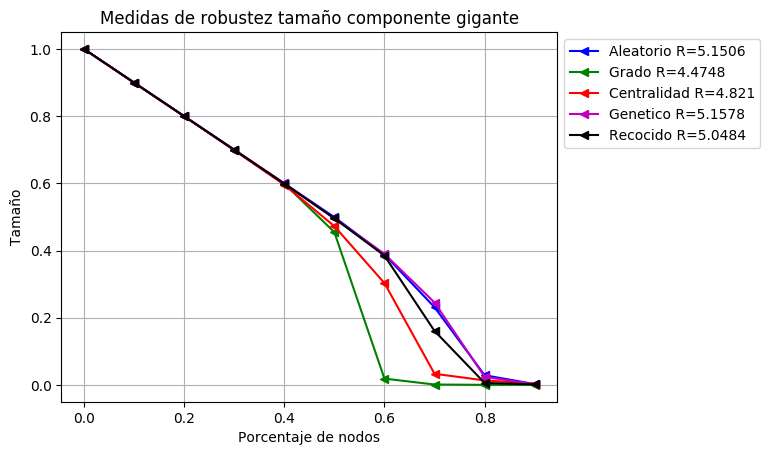
\includegraphics[scale=0.7]{Capitulo5Robustez/imagenes/grafica_GC20180510_143549SmallWorld5000NodesRewire01.png}
    \caption{Medida componente de gigante}
    \label{figure:smallWorldGC}
\end{figure}


\begin{figure}[H]
    \centering
    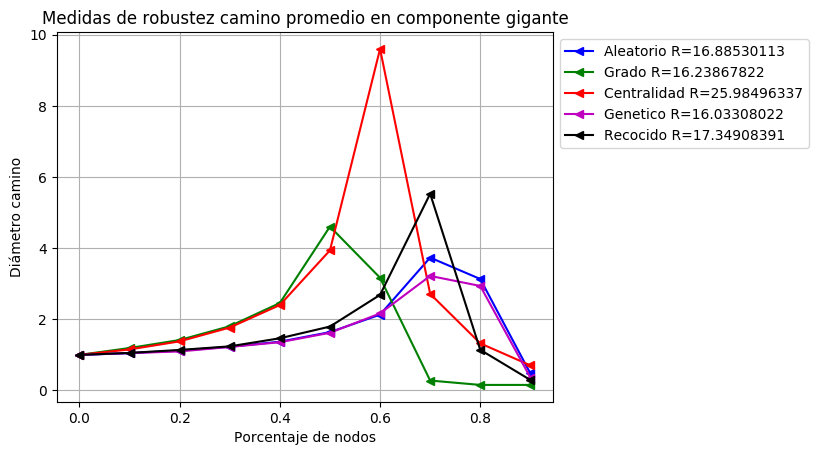
\includegraphics[scale=0.7]{Capitulo5Robustez/imagenes/grafica_APL20180510_143549SmallWorld5000NodesRewire01.png}
    \caption{Medida componente de promedio de camino más cortos}
    \label{figure:smallWorldAPL}
\end{figure}

En el caso de las redes de mundo pequeño, la medida que cobra importancia es el promedio de los caminos más cortos, ya que al destruir nodos por centralidad se pierde la propiedad de conservar un valor promedio pequeño de distancia más corta entre un par de nodos cualesquiera.


\subsection{Pruebas red aleatoria}


\begin{figure}[H]
    \centering
    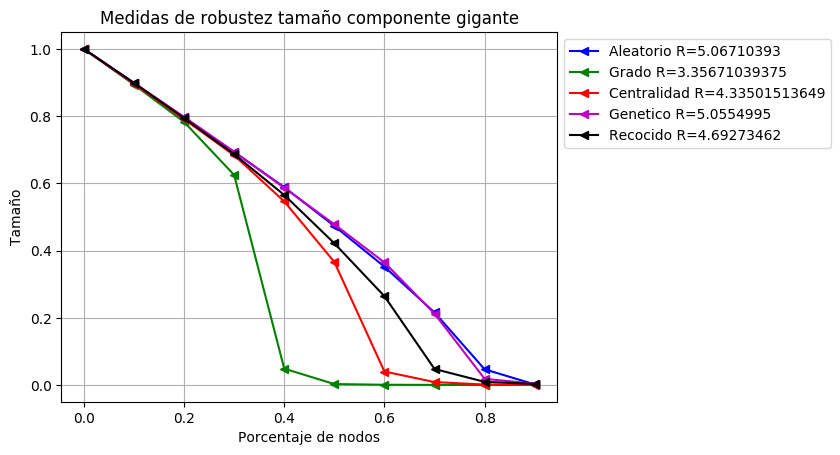
\includegraphics[scale=0.7]{Capitulo5Robustez/imagenes/grafica_GC20180501_072543Random1991Nodes5939.png}
    \caption{Medida componente de gigante}
\end{figure}


\begin{figure}[H]
    \centering
    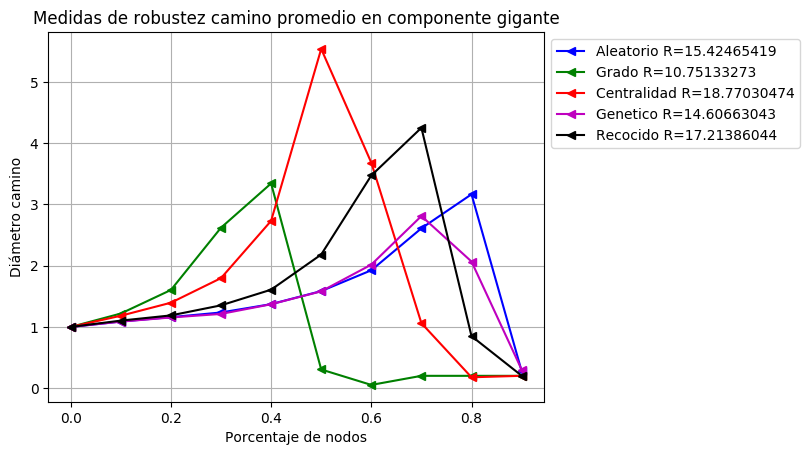
\includegraphics[scale=0.7]{Capitulo5Robustez/imagenes/grafica_APL20180501_072543Random1991Nodes5939.png}
    \caption{Medida componente de promedio de camino más cortos}
\end{figure}

En las redes aleatorias, el ataque por centralidad tiene el mismo efecto que las redes de mundo pequeño.


\subsection{Prueba en red observada Celengs}

\begin{figure}[H]
    \centering
    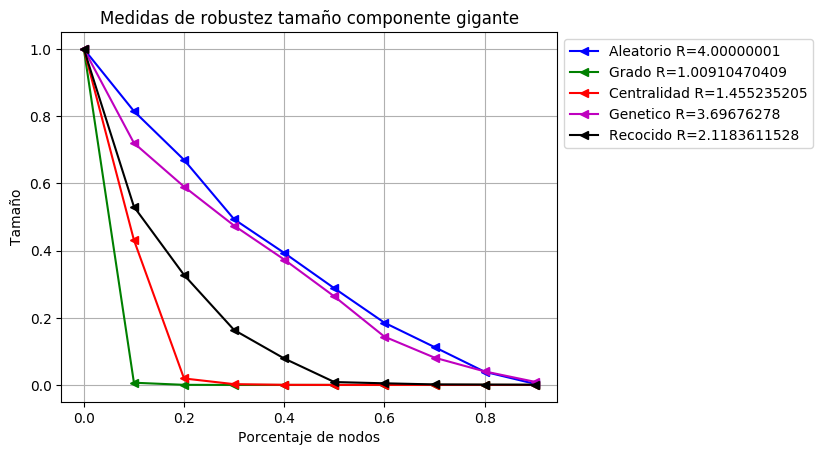
\includegraphics[scale=0.7]{Capitulo5Robustez/imagenes/grafica_GC20180508_020345Celengs.png}
    \caption{Medida componente de gigante}
\end{figure}


\begin{figure}[H]
    \centering
    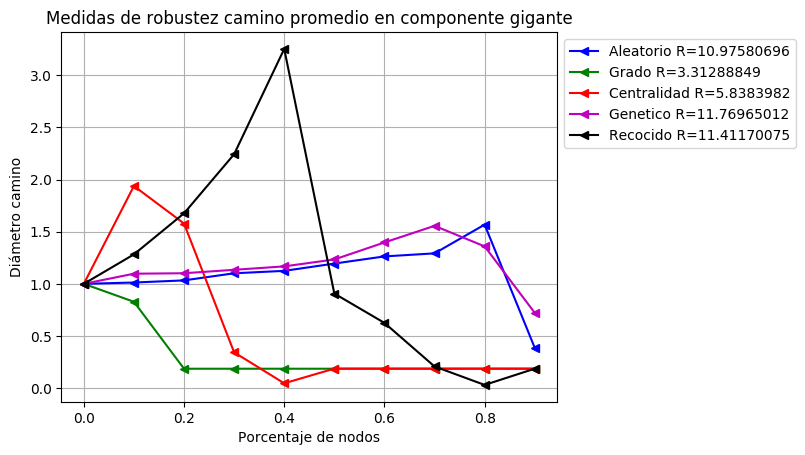
\includegraphics[scale=0.7]{Capitulo5Robustez/imagenes/grafica_APL20180508_020345Celengs.png}
    \caption{Medida componente de promedio de camino más cortos}
\end{figure}


En el caso de esta red observada, se observa que tiene la presencia de hubs, ya que al eliminar nodos por su grado, el tamaño del componente gigante se ve reducido considerablemente.

\subsection{Prueba red fractal}

\begin{figure}[H]
    \centering
    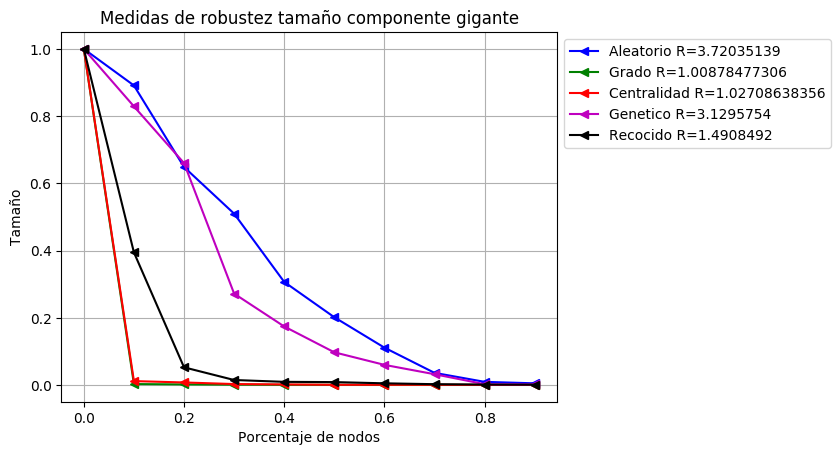
\includegraphics[scale=0.7]{Capitulo5Robustez/imagenes/grafica_GC20180501_151350floweru1v3.png}
    \caption{Medida componente de gigante}
\end{figure}


\begin{figure}[H]
    \centering
    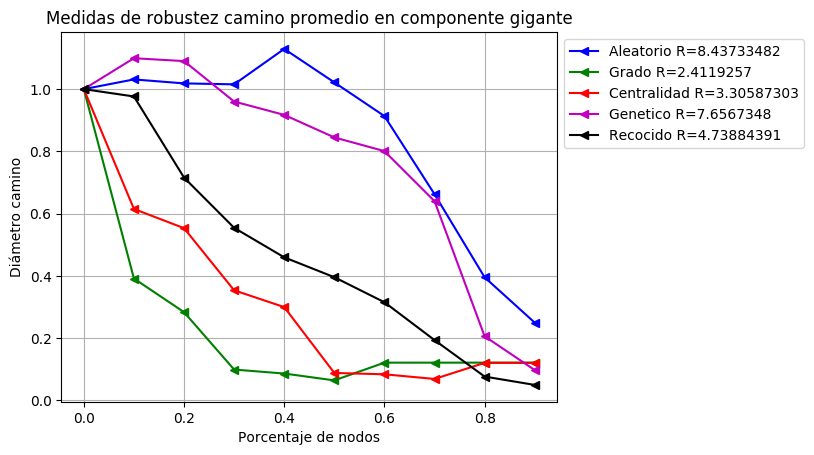
\includegraphics[scale=0.7]{Capitulo5Robustez/imagenes/grafica_APL20180501_151350floweru1v3.png}
    \caption{Medida componente de promedio de camino más cortos}
\end{figure}

En el caso del red fractal, la estrategia de ataque más eficiente es la de centralidad. Esto se explica debido a que los fractales se generan iterativamente a partir de los nodos de las generaciones anteriores, los cuales pasan a ser parte de los caminos más cortos entre cualquier par de nodos.